\documentclass[buriama8_dp.tex]{subfiles}
\begin{document}

\chapter{Experiments}

We conducted both simulated experiments and experiments on a real robotic arm to test our solution and its implementation. First, we experimentally tested the new Jacobian control mechanism we implemented, to determine if it was usable for our solution. Then, the coverage path planning algorithms were tested in simulation first. Finally, the compact space heuristic algorithm was put to the test both in simulation and with the real arm.

\section{Benchmark environment}
\label{sec:exp_cpp_env}

We created a benchmark environment representing an obstacle in front of the robot. The environment is represented by a grid \(10 \times 10 \times 5\) cells. We also tested the algorithms in free space, to see if they can produce optimal (non-overlapping) paths at least in the simplest of environments, despite their heuristic nature.

The environment contains two obstacles, a floor-standing object and an overhang above the object, with enough space for the robot to pass through. A single plane, the second nearest vertical plane to the robot, extracted from the full 3D environment is used as the 2D benchmark for the coverage algorithm. The planar environment is illustrated in Figure~\ref{fig:2d_env}.

\begin{figure}[htp]
  \centering
  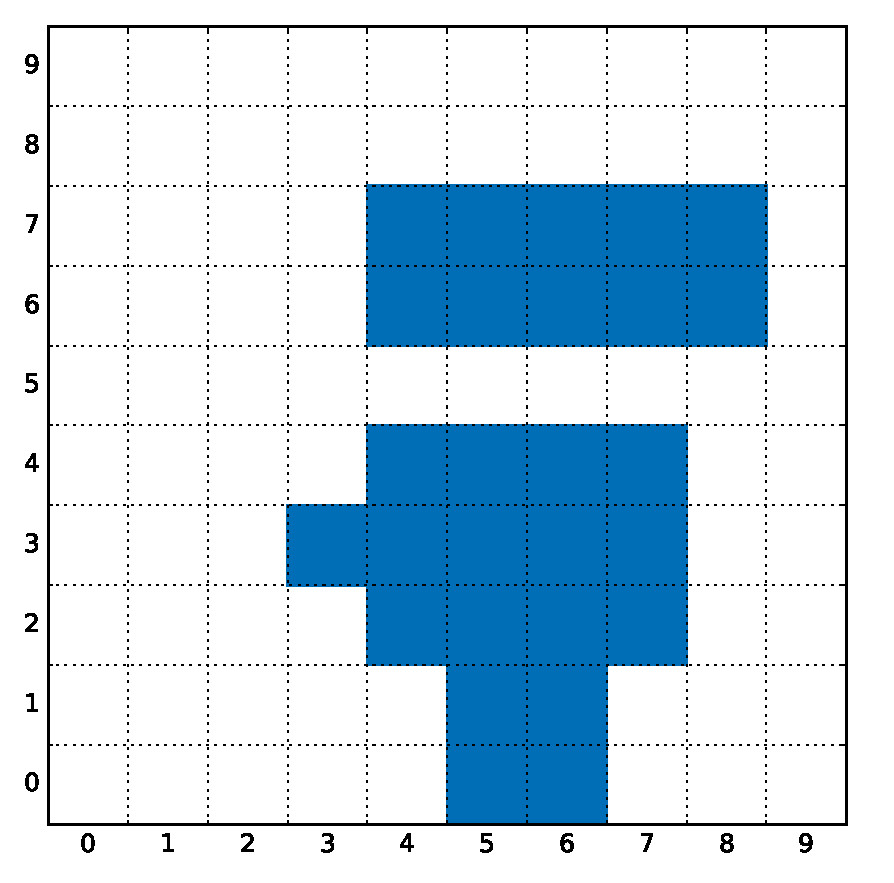
\includegraphics[width=7cm]{2d_coverage_env.pdf}
  \caption[2D benchmark environment]{The 2D benchmark environment for CPP algorithms. The environment is depicted as a vertical slice as seen by the robot; the \uvz{floor} is at the bottom}
  \label{fig:2d_env}
\end{figure}

In simulating coverage algorithms we ignore the potential arm collisions with previously discovered obstacles. This is accounted for when we simulate the whole arm.

\section{Simulated coverage algorithms}
\label{sec:exp_sim_coverage}

To test the performance of CPP algorithms we implemented, we performed experiments to determine how well the methods perform in unknown environments in both 2 and 3 dimensions. Each of the algorithms was run in empty 2D environment to test it in the simplest setting, followed by a run in the benchmark environment described in Section~\ref{sec:exp_cpp_env} Because of the generalization scheme used to adapt the algorithm to explore 3D space, 2D environment is represented in 3D as a grid with only one depth layer.

\subsection{Two dimensions}
\label{subsec:2d_sim}

\subsubsection{Random algorithm}
To establish a baseline to test against, we first tested a basic random algorithm. One of the generated paths can be seen in Figure~\ref{fig:rand_2d_coverage}.

\begin{figure}[htp]
  \centering
  \begin{subfigure}[t]{0.49\textwidth}
    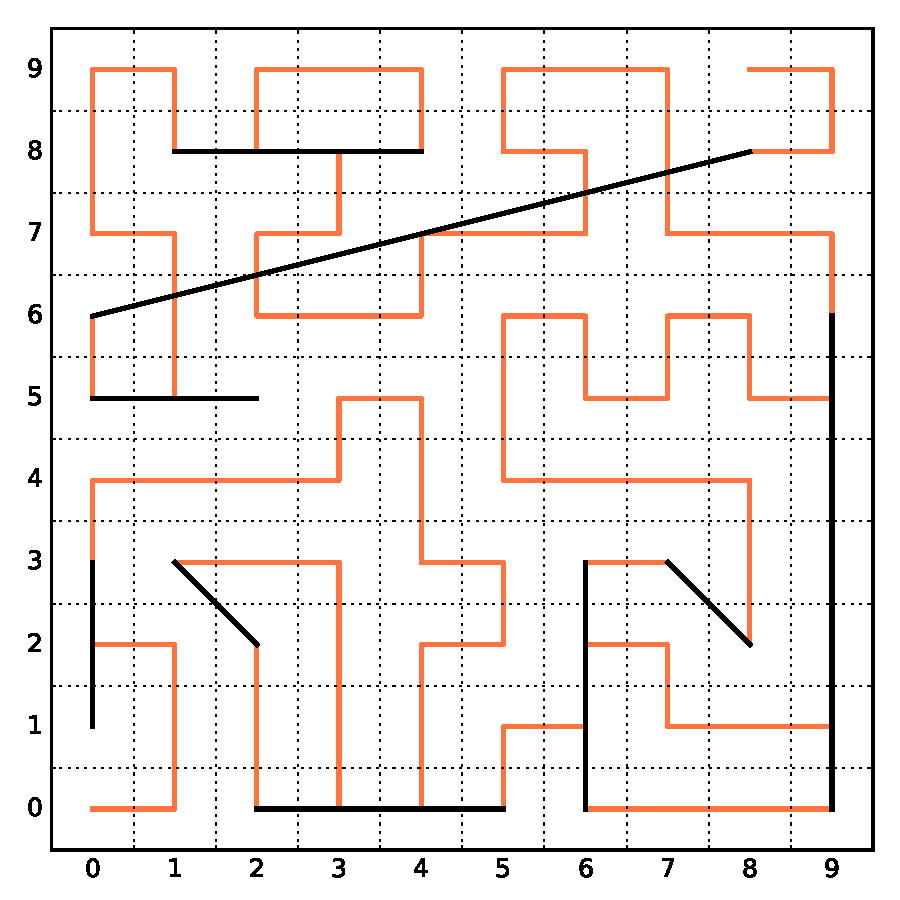
\includegraphics[width=\textwidth]{2d_coverage_random_empty.pdf}
    \caption{}
    \label{fig:rand_2d_empty}
  \end{subfigure}
  \begin{subfigure}[t]{0.49\textwidth}
    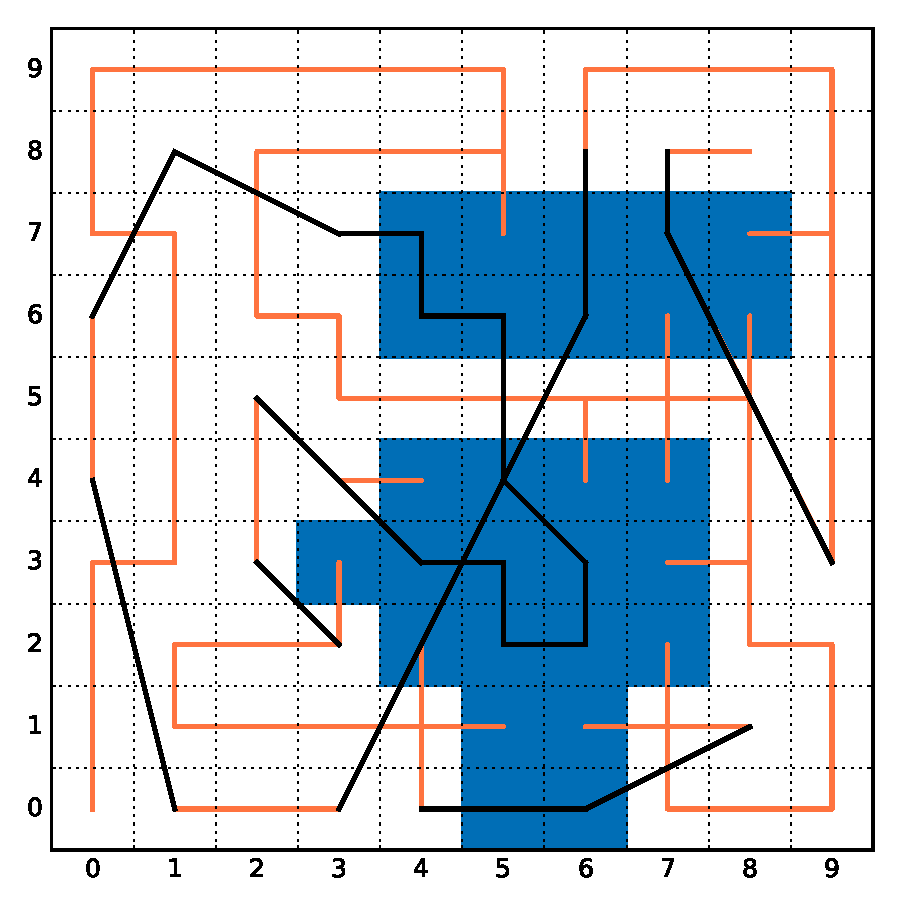
\includegraphics[width=\textwidth]{2d_coverage_random.pdf}
    \caption{}
    \label{fig:rand_2d_env}
  \end{subfigure}
  
  \caption[Coverage path -- random algorithm in 2D]{Coverage path generated by a random algorithm in an empty (a) and in the benchmark environment (b). The path starts at \([0,0]\) and is depicted in orange, with transitions to nearest unexplored field depicted in black. The global transitions sometimes cover the previous ordinary ones}
  \label{fig:rand_2d_coverage}
\end{figure}

The algorithm randomly chooses an unexplored neighboring field; if no such is available, it goes to the nearest unexplored field. The lengths of the displayed paths are 12\,m in the empty and 13\,m in the benchmark environment, while the mean lengths of paths generated over five trials were 11.7\,m (min. 11.4\,m, max. 12.1\,m) and 12.8\,m (min. 12.5\,m, max. 13\,m), respectively.

\subsubsection{Compact space heuristic}
Running the compact space heuristic algorithm in the 2D environment, we obtained paths depicted in Figure~\ref{fig:heur_2d_coverage}.

\begin{figure}[htp]
  \centering
  \begin{subfigure}[t]{0.49\textwidth}
    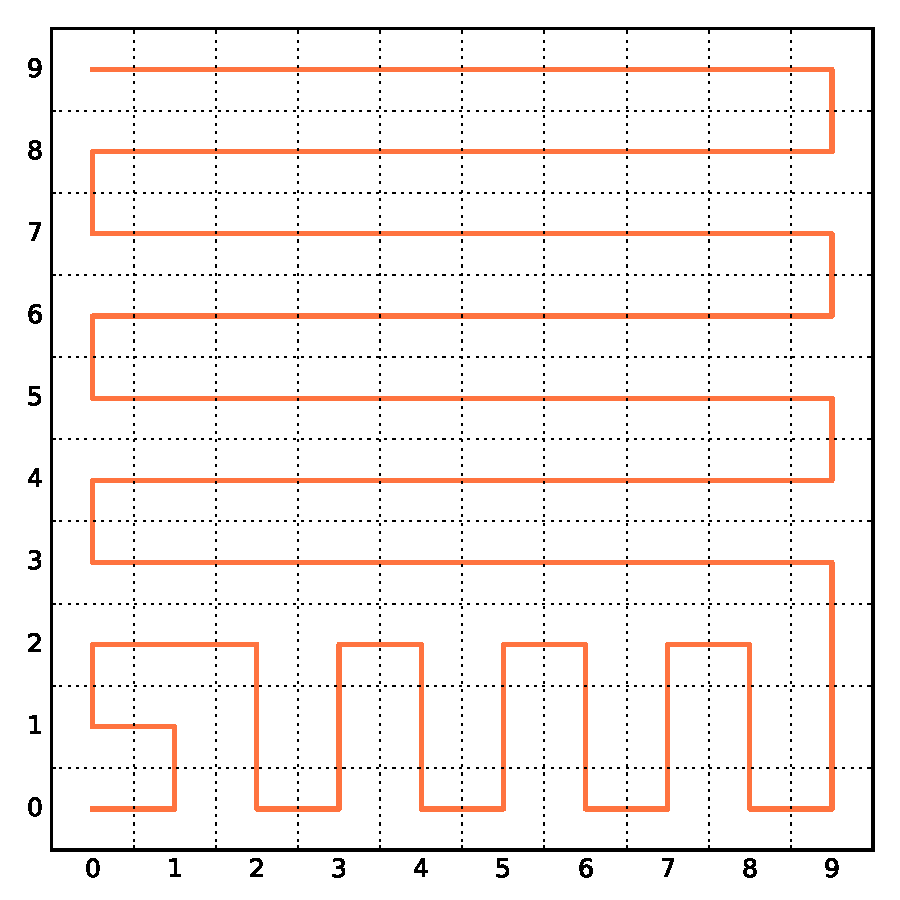
\includegraphics[width=\textwidth]{2d_coverage_heur_empty.pdf}
    \caption{}
    \label{fig:heur_2d_empty}
  \end{subfigure}
  \begin{subfigure}[t]{0.49\textwidth}
    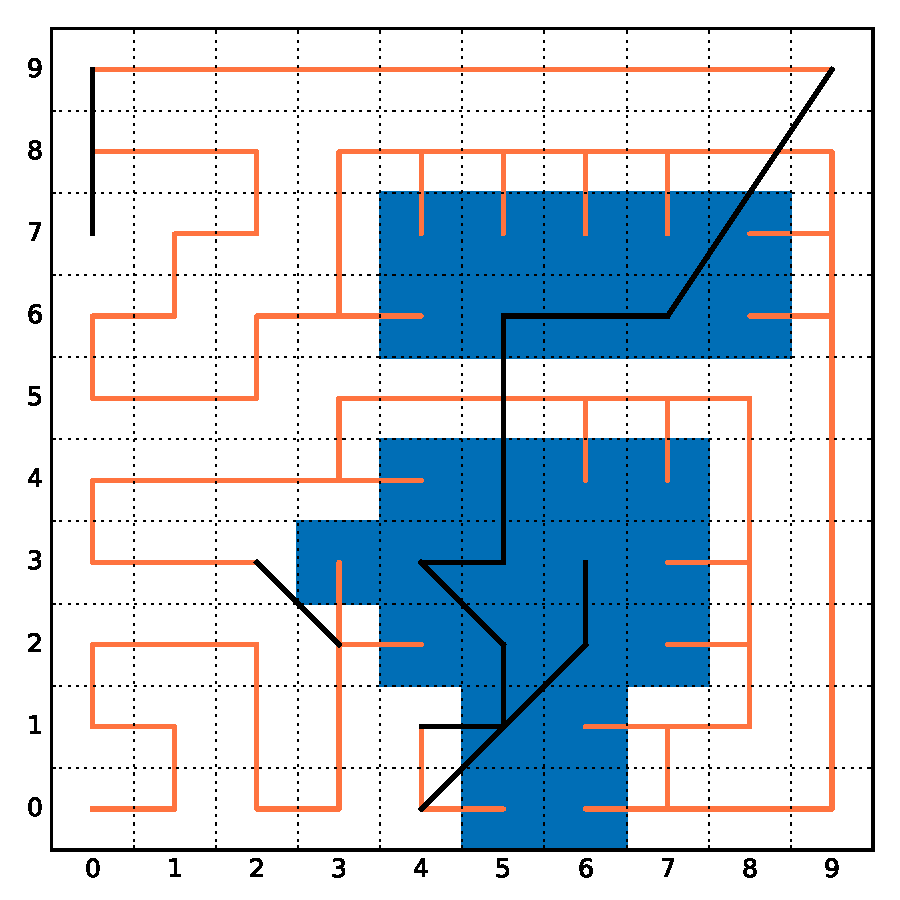
\includegraphics[width=\textwidth]{2d_coverage_heur.pdf}
    \caption{}
    \label{fig:heur_2d_env}
  \end{subfigure}
  
  \caption[Coverage path -- compact space heuristic in 2D]{Coverage path generated by the compact space heuristic in an empty (a) and in the benchmark environment (b). The path starts at \([0,0]\) and is depicted in orange, with transitions to nearest unexplored field depicted in black}
  \label{fig:heur_2d_coverage}
\end{figure}

The results in empty space are reasonable. The generated path closely resembles the boustrophedon pattern used in human-designed algorithms. The already explored space is kept compact, as was the aim of the heuristic. The length of the generated path is 9.9\,m, which is the optimal value since no cell was explored twice. This is allowed by the even size of the environment; in case of odd environment width, the lower zig-zag terminates in the lower-right corner and the robot then has to return back to the yet unexplored portion of the environment, traveling through the already known fields again.

In the benchmark environment, we can see that the path starts the same as in the empty environment. When the obstacle is encountered, we can identify the algorithm following the other incentive it has -- exploring space near known obstacles. This leads to obstacle-circling, after which the obstacle limits are quickly determined. A snapshot from exploration progress is displayed in Figure~\ref{fig:heur_fn}. The length of the path is 12.5\,m, better than any run of the random algorithm.

\begin{figure}[htp]
  \centering
  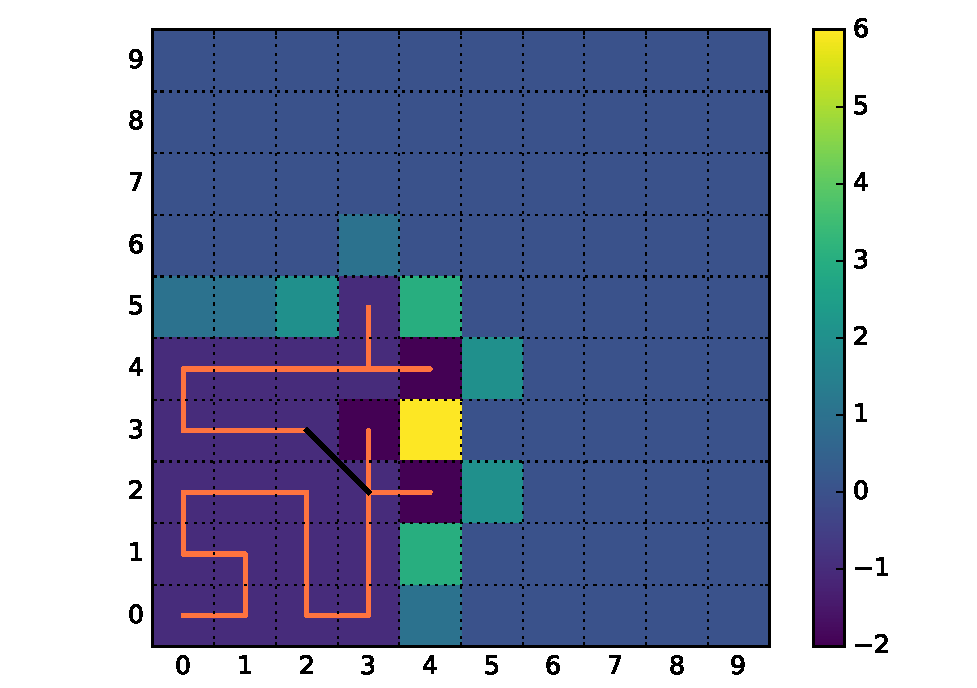
\includegraphics[width=8cm]{expl_heuristic_fn.pdf}
  \caption[Inner state of heuristic algorithm]{Intermediate state of exploration of the benchmark environment by the compact space heuristic. The tool is now at position (3, 5). The fields with value \(-2\) (dark blue) are already discovered obstacles, the fields with \(-1\) were identified as free. The other values represent the value of the heuristic function in the cell. As we can see, the robot will continue right as cell (4, 5) is adjacent to an obstacle, as opposed to (2, 5)}
  \label{fig:heur_fn}
\end{figure}


\subsubsection{Neural network}
The results of the NN algorithm are presented in Figure~\ref{fig:nn_2d_coverage}.

\begin{figure}[htp]
  \centering
  \begin{subfigure}[t]{0.49\textwidth}
    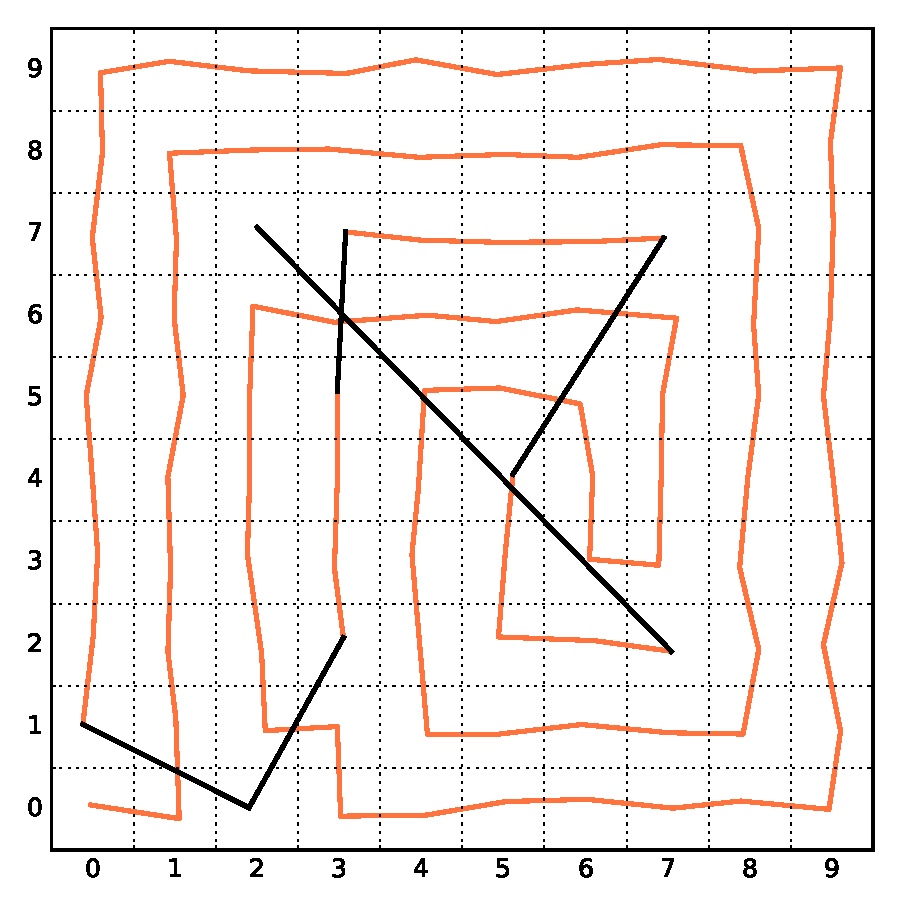
\includegraphics[width=\textwidth]{2d_coverage_nn_empty.pdf}
    \caption{}
    \label{fig:nn_2d_empty}
  \end{subfigure}
  \begin{subfigure}[t]{0.49\textwidth}
    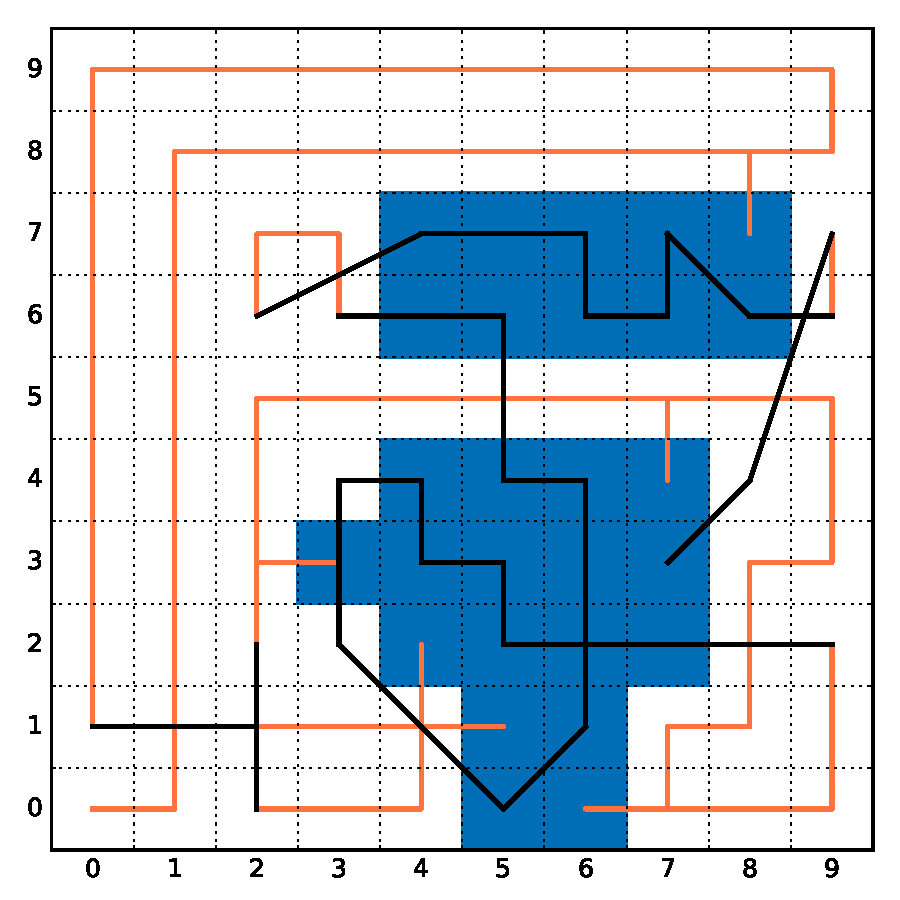
\includegraphics[width=\textwidth]{2d_coverage_nn.pdf}
    \caption{}
    \label{fig:nn_2d_env}
  \end{subfigure}

  \caption[Coverage path -- neural network in 2D]{Coverage paths generated by the neural network algorithm, in empty environment (a) and the benchmark environment (b)}
  \label{fig:nn_2d_coverage}
\end{figure}

\begin{figure}[htp]
  \centering
  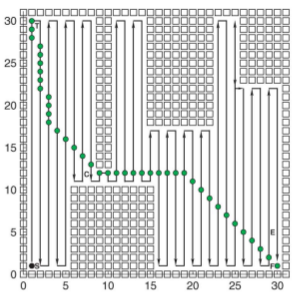
\includegraphics[width=4cm]{nuronet.png}
  \caption[Original neural network path]{The path obtained by the authors of the algorithm (image taken from \cite{neural})}
  \label{fig:nn_article}
\end{figure}

The NN algorithm tests have been described by its authors, an example of a path generated by the original implementation is presented in Figure~\ref{fig:nn_article}. The trajectory we obtained is completely different, even with the algorithm without the modifications described in \ref{subsec:impl_neuro}. No tuning of parameters achieved such path. The authors do not give any details on their implementation of the network dynamics simulation, and that may be the reason for such failure. We present an insight into the algorithm decision making in Figure~\ref{fig:nn_fn}, where the neural activity evolution during exploration is presented. More detail on the activity development can be found in the original article \cite{neural}. 

The path output by our implementation fails to cover even empty environment without overlaps. The path is 11.11\,m long and includes 5 transitions to the nearest unexplored cell.

In the benchmark environment, the generated coverage path is 11.75\,m long, surprisingly less than in the case of the compact space heuristic. The reason is that the path in the compact heuristic contains many simple moves hitting the obstacles and then returning back to the free space. In the NN case, most of the obstacles are visited by the global transitions, which follow the shortest paths, decreasing the total path length. The global transitions are driven by motion planning, and as such their preparation and execution is more time-consuming than that of the simple motions from one cell to its neighboring cell.

\begin{figure}[ht]
  \centering
  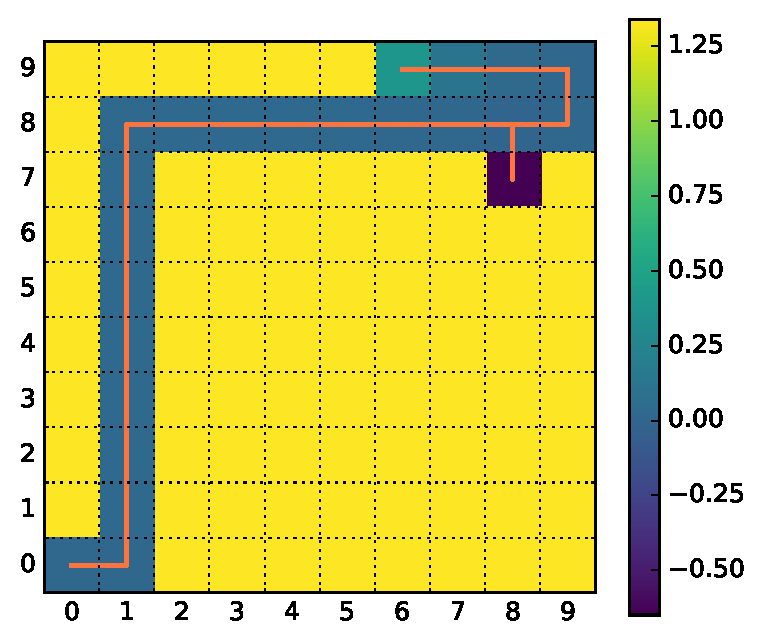
\includegraphics[width=7cm]{expl_nn_fn.pdf}
  \caption[Internal state of neural network algorithm]{The neural activity in the network after a few algorithm steps. The deep blue obstacle and yellow unexplored area are pulled down and up by the external inputs. The robot is at position (6,9); we can observe the neural activities in the robot's trail decaying after setting the external input to zero}
  \label{fig:nn_fn}
\end{figure}


In conclusion, the compact space heuristic provided the most efficient solutions to path planning in 2D. The neural network algorithm produced competitive trajectories that however contained many global transfers and were thus more complicated and time-consuming.

\subsection{Three dimensions}
\label{subsec:3d_sim}

The results of running the coverage algorithms are shown in Figure~\ref{fig:heur_3d_coverage}. We did not evaluate the random planner in 3D as the performance of the 3D instance should, due to the generalization scheme employed, be directly related to the performance in 2D, where it was outperformed completely. 

\begin{figure}[tp]
  \centering
  \begin{subfigure}[t]{0.48\textwidth}
    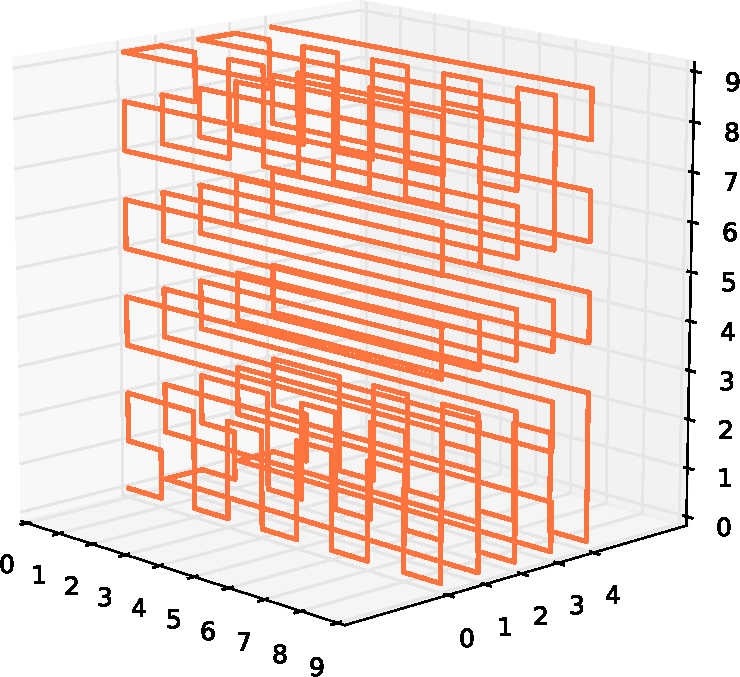
\includegraphics[width=\textwidth]{3d_coverage_heur_empty-cropped.pdf}
    \caption{}
    \label{fig:heur_3d_empty}
  \end{subfigure}
  \;
  \begin{subfigure}[t]{0.48\textwidth}
    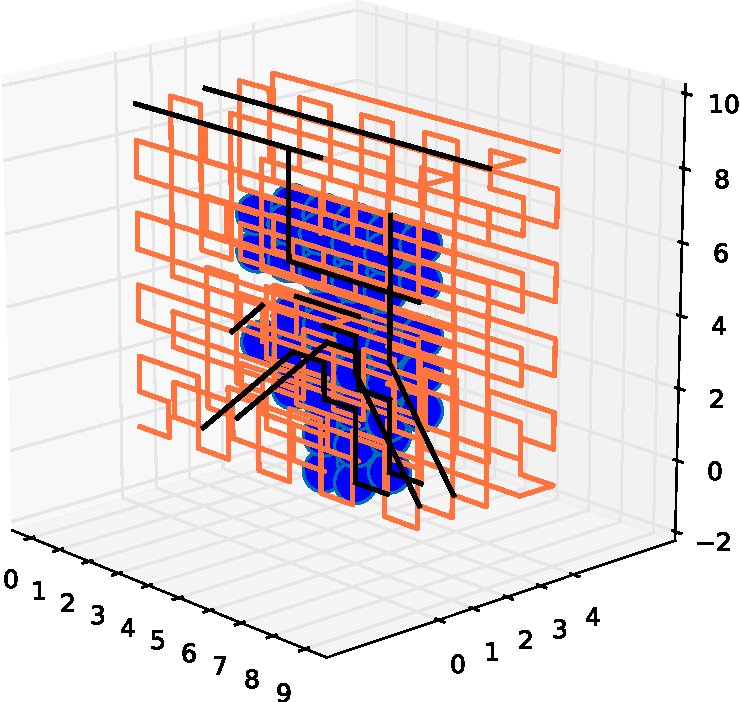
\includegraphics[width=\textwidth]{3d_coverage_heur-cropped.pdf}
    \caption{}
    \label{fig:heur_3d_env}
  \end{subfigure}
  
 \begin{subfigure}[t]{0.48\textwidth}
    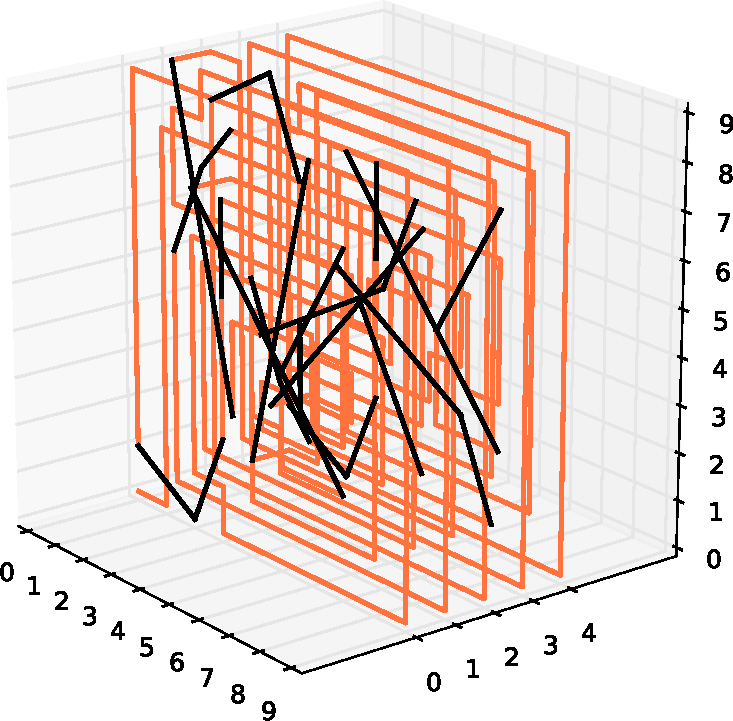
\includegraphics[width=\textwidth]{3d_coverage_nn_empty-cropped.pdf}
    \caption{}
    \label{fig:nn_3d_empty}
  \end{subfigure}
  \;
  \begin{subfigure}[t]{0.48\textwidth}
    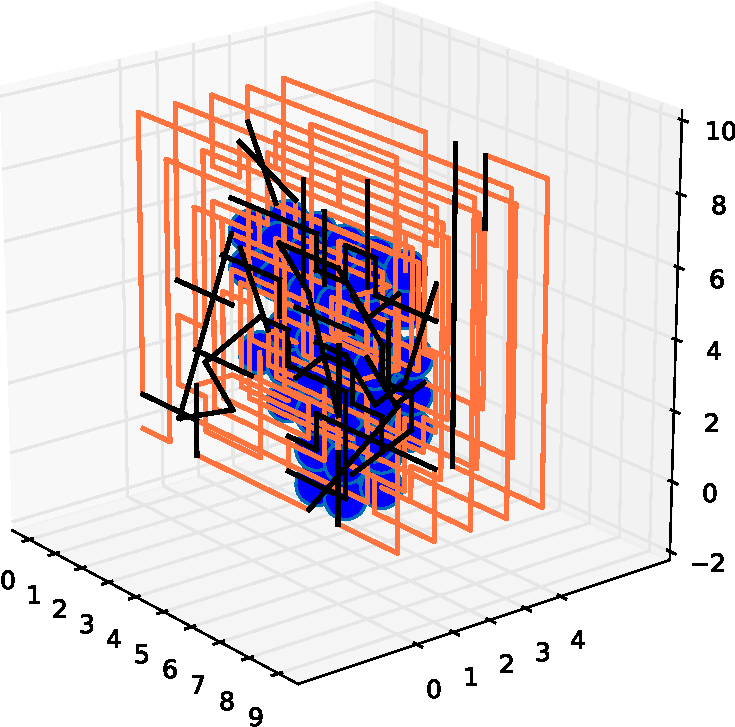
\includegraphics[width=\textwidth]{3d_coverage_nn-cropped.pdf}
    \caption{}
    \label{fig:nn_3d_env}
  \end{subfigure}
  
  \caption[Coverage path -- compact space heuristic in 3D]{The coverage path generated  by compact space heuristic in 3D in (a) empty space and (b) benchmark environment. The path by NN algorithm is in subfigures (c) and (d) in empty and in the benchmark environment, respectively. The obstacles are represented by spheres at the given point}
  \label{fig:heur_3d_coverage}
\end{figure}

\subsubsection{Compact space heuristic}
Expectedly, the algorithm runs in 3D space as well as in two dimensions. In both cases, we can observe the layers in which the environment has been explored. In the empty environment, the algorithm starts and ends on opposite sides, and thus the layers are identical, only mirrored. The found path in Figure~\ref{fig:heur_3d_empty} is again optimal with length of 49.9\,m.

When obstacles are present, the coverage path is different in each layer partly because of the varying obstacles, partly because of different entry points, as one layer starts precisely where the other has ended. The path in Figure~\ref{fig:heur_3d_env} is 56.3\,m long.

\subsubsection{Neural network}
The results of the NN algorithm are irregular, as the algorithm proceeds in a sort of a spiral, and thus ends in one layer and starts in the other in central locations. The path in Figure~\ref{fig:nn_3d_empty} is 55.2\,m long and contains too many global transitions.

In the environment with obstacles, the generated path in Figure~\ref{fig:nn_3d_env} is 57\,m long.


\subsection{Conclusions}
\label{subsec:alg_concl}

The results of our experiments are summarized in Table~\ref{tab:len}.

\begin{table}
\begin{ctucolortab}
\begin{tabular}{l|cc}
\bfseries Algorithm & \bfseries Compact space & \bfseries Neural network \\\Midrule
2D free & \textbf{9.9\,m} & 11.1\,m\\
2D & 12.5\,m & 11.75\,m\\
3D free & \textbf{49.9\,m} & 55.2\,m\\
3D & 56.3\,m & 57\,m
\end{tabular}
\end{ctucolortab}
\caption{Generated path lengths in the simulated experiments. Numbers in bold represent known optimal solution}
\label{tab:len}
\end{table}

In all cases, except in the 2D benchmark environment, the compact space heuristic provided more efficient path than the neural network. In the one case, it was at the expense of many global transitions. Hence, we will use the compact space heuristic as the exploration algorithm for the rest of the experiments.


\section{Simulated arm experiments}
\label{sec:exp_sim_arm}

\subsection{Moving the arm}
\label{subsec:exp_move_sim}

In Sections \ref{subsec:motion_planning} and \ref{subsec:no_plan}, we mention two ways of driving the robot: motion planning and Jacobian transformation. Both have their advantages and disadvantages. We tested them by running the algorithm with each as the robot driving function. We used only the simulated arm at first to protect the hardware from unfortunate accidents.

We let the simulated arm explore empty space. We evaluated the failures of the movement, such as getting stuck, and the smoothness, precision and optimality of the overall path.

The error measurements both in this section and in Section~\ref{subsec:exp_move_real}, which describes the errors measured on the real arm, are based on position reported by the robot. The joint position sensors in this simulation have only rounding errors. The real arm position is reported by rotation encoders in arm actuators, that have angular resolution of \(0.068\degr\) to \(0.047\degr\) (three different actuator types are used in the arm), with unknown error \cite{jaco_joint_spec}.

The motion planning method is very reliable in always reaching the desired target pose, and reaching it precisely, when performing a step in the algorithm in the empty environment. In the test run, all the steps were carried out successfully. The planning took hundreds of milliseconds for each step. Even when using the TRAC-IK solver, sometimes a joint configuration  very different from the current one was found as the IK solution by the solver. The planner then had no other option than to plan a more complicated path, perhaps rotating the first joint by \(180\degr\).

That being said, the planning success rate dropped drastically when obstacles were present in the planning scene, and in tight restrictions, it often failed completely as the planner was unable to find a way out of the restriction. Mere proximity of obstacles also posed a challenge to the motion planner. If the path was found, which occured as infrequently as once in ten planning trials, the generated paths were messy to say the least. An example of such path can be found in Figure~\ref{fig:collision_plan}. In some instances, alarmingly, a plan that caused collision was allowed, because the discretized poses in which collisions were checked skipped the one in collision. The overlap was only very small and short, but could cause a problem in real arm operation.

\begin{figure}[htp]
  \centering
  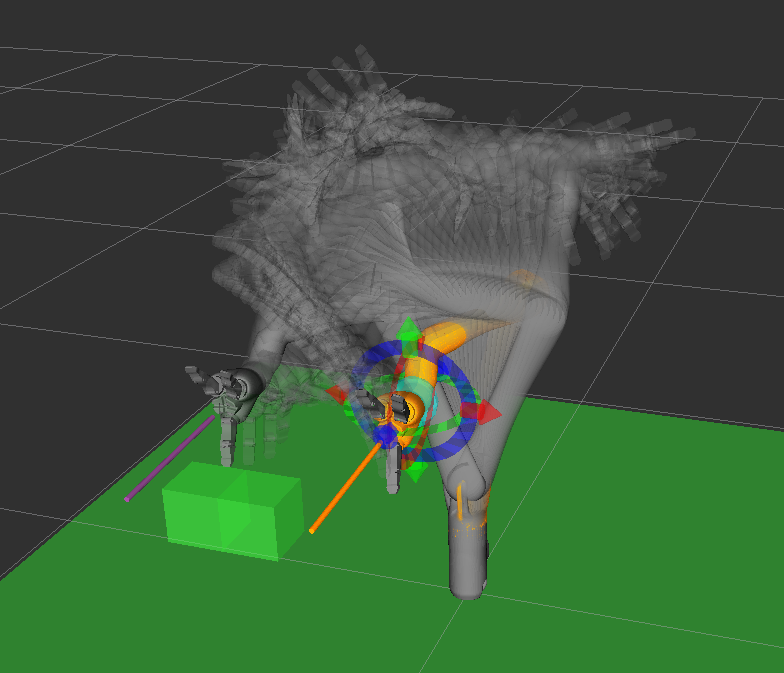
\includegraphics[width=7cm]{wrong_plan_close_obstacle.png}
  \caption[Obstacle avoiding motion plan]{An example of a not at all optimal plan, the only one found due to a close obstacle only after five planning attempts. The start state is solid grey, the requested target is orange. The planned path is visualized as a sequence of semi-transparent intermediate arm states}
  \label{fig:collision_plan}
\end{figure}


The Jacobian method is extremely fast. The pause at each step is only a few milliseconds, the arm seemingly does not stop at all.  During the tests, we noticed slight deviations of the arm from the trajectory it was to follow, and conducted further experiments to determine their nature.

\subsection{Jacobian control precision}
\label{subsec:label}


We tested the control algorithm by driving the arm across its workspace along the \m x axis. The arm followed the given trajectory with tolerance of 2\,mm. To further improve the here completely satisfactory result, we turned on the error correcting term described in Section~\ref{subsec:impl_drv_jacob}. The precision then got near perfect, with error of at most 0.4\,mm. The errors are depicted in Figure~\ref{fig:err_jac_sim}. 

\begin{figure}[ht]
  \centering
  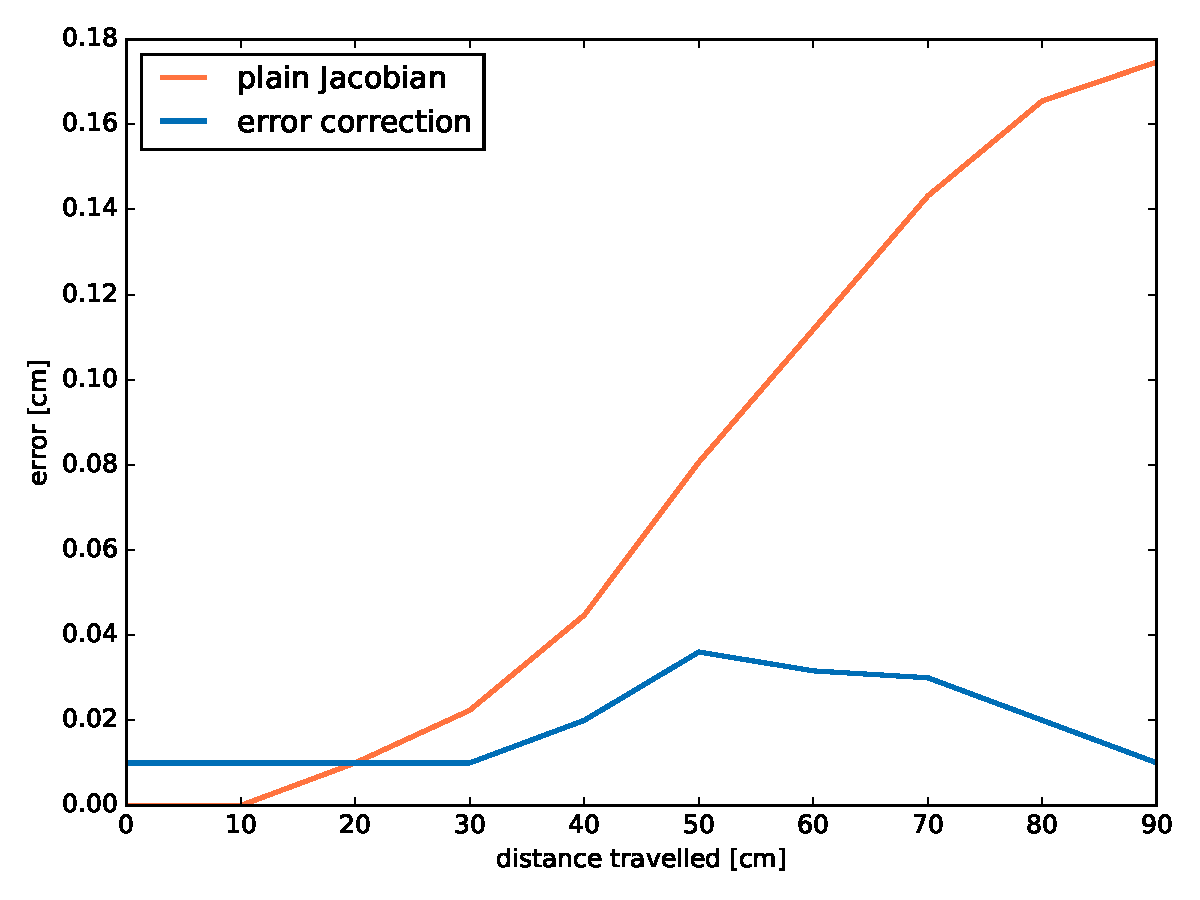
\includegraphics[width=7cm]{jacob_error_sim.pdf}
  \caption{Position error during simulated test drive}
  \label{fig:err_jac_sim}
\end{figure}

The error is probably caused by the numerical error attained in integrating the speeds in discrete steps in the control loop.

In some cases, mostly directly in front of the arm base, a near singularity is reached. The tested trajectory passes in front of the arm's base at 45\,cm. We can see the effects of the singularity in the plot. While we attempt to solve things by slowing the arm down (see the implementation details in Section~\ref{subsec:impl_drv_jacob}), in some configurations, we get so close to the exact singular configurations that no slow-down helps. The driving algorithm identifies such situations and reports failure to higher layers.

The final combined solution described in Section~\ref{subsec:impl_drv} proved to combine the best properties of both the methods. The fallback to planning is used exactly when necessary. In some cases, however, the Jacobian motion stops due to a collision warning, but it stops too close to the obstacle. Then, even planning fails to move the arm to explore the next cell and it is misclassified as unreachable. This results in false positive obstacles identified in the environment.

\subsection{Exploring 3D environment}
\label{subsec:sim_arm_cover}

We tested the final coverage algorithm first in the simulator. We ran it first in empty environment, then in the benchmark environment. The benchmark environment was simulated by publishing false force readings when the arm explored an occupied point.

Initially, we ran the algorithm without checking for collisions between the stick and other explored cells, to verify that at least the simplified version can be solved. We ran the algorithm several times, as the motion planning is not deterministic.

In every run in the free environment, a few cells were reported as unreachable due to planning algorithm failure. When the arm was close to a collision cube of another non-explored cell, the motion planning failed frequently. This was the case very infrequently, though. The arm itself stays safely away from the obstacles, and only the stick is meant to get so close. However, once a cell is marked unreachable and its collision cube left in the environment, the cells that require the arm to get close to the original cell are reported as unreachable as well due to the planning issues. The effect propagates, making a portion of the environment unreachable.

\begin{figure}[ht]
  \centering
  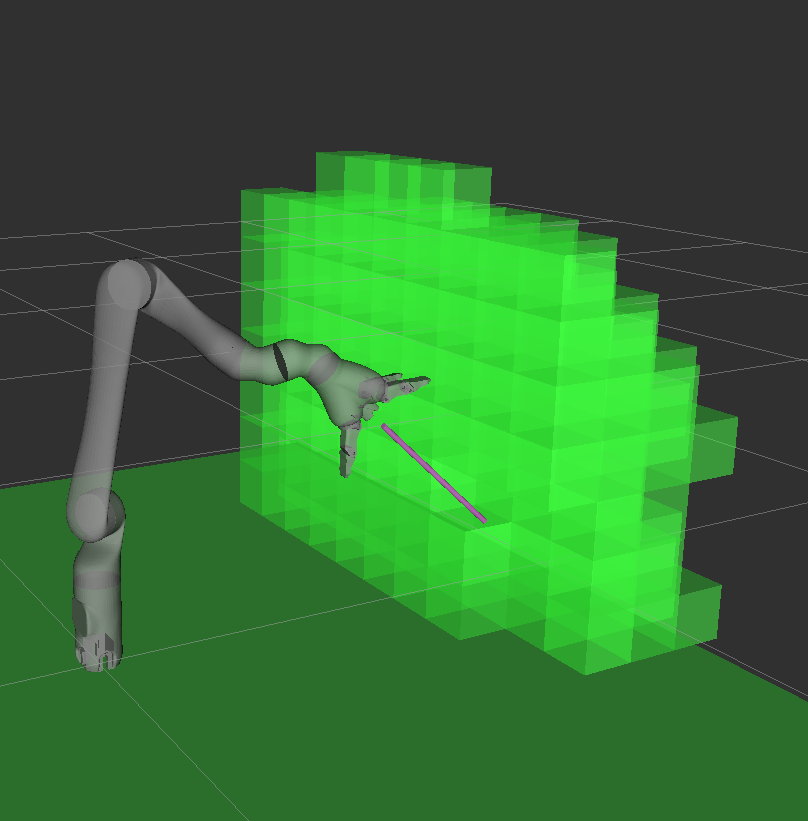
\includegraphics[width=7cm]{sim_exploring2.png}
  \caption[Simulated arm exploring environment]{The simulated arm with the collision model of the sensing tool attached exploring the environment in simulation}
  \label{fig:sim_expl}
\end{figure}

Once the collision stick is attached to the robot model, the effects of obstacle proximity planning issues magnify, as the stick is close to the other collision objects all the time. The Jacobian control works as expected, but virtually all planning requests fail, marking large portions of the environment as unreachable.

The sole cause of the issues is the motion planner. Its sampling of states around the start and goal states fails utterly when it needs to pass through a restriction where there is very low probability of sampling a state that is both valid and then leads to the other state. The high efficiency of the planners in obstacle-free environment is given by the path simplification step, where the trajectories from start to end state, usually containing hundreds of states, are often simplified to direct trajectory from the start to the end state.

We also tested several different planners, to no improvement. If the target pose is in restricted space, the unidirectional planners need to be extremely lucky to sample a state from which the final state is reachable. Bidirectional planners fail to sample any states reachable from the end state directly. Even RRT planners that boast of good configuration state exploration cannot sample any such states.

The issues could in the future be resolved by using another motion planner, perhaps one specially designed to work in this case that could exploit the structure in the problem, like the knowledge that we are dealing with a grid of cubes.

\subsection{Conclusions}
\label{subsec:exp_sim_concl}

We tested the arm control in simulated environment. The motion control works as expected in empty space; when the arm gets close to colliding with a collision object, the planning capabilities are drastically reduced. Planning arm motion in the exploration algorithm is usable when stick collision checking is omitted. In that case, the arm managed to explore the environment with misclassifying only a few cells as unreachable.

Further work is necessary to make the exporation more robust, mainly in the field of motion planning. We need to plan motions in tightly constrained spaces, but we have additional knowledge about the space.


\section{Real arm experiments}
\label{sec:exp_real_arm}

Experiments in the simulator are safe and very valuable during development, where we can focus on testing the code rather than checking if the arm is going to be safe. Nonetheless, real world experiments are absolutely necessary, as the system is in the end meant to run on a real rescue robot.

\subsection{Moving the arm}
\label{subsec:exp_move_real}

We aimed to confirm the results of movement simulation on the real hardware. Motion planning exhibited the same behavior as in the simulation. It worked reliably, but in some seemingly random cases, a very complicated plan was generated. These complicated motion plans threaten, among others, the cable linking the sensing tool to the host computer.

When we repeated the Jacobian control test we used with the simulated arm, we discovered that the real arm deviates from the intended trajectory significantly. After following the same trajectory, the arm deviated 6\,cm in \m y and 4\,cm in \m z direction. We assume the error was given by neglecting the arm dynamics, assuming the given joint velocity can be reached immediately by the arm.

This high error gave us the incentive to implement the regulator described in \ref{subsec:impl_drv_jacob} that would correct the errors. The results were excellent, with maximum error along the path 2\,cm and final error 4\,mm. The errors are depicted in Figure~\ref{fig:err_jac_real}. We then re-ran the simulated experiment with correction to complete the results.

\begin{figure}[ht]
  \centering
  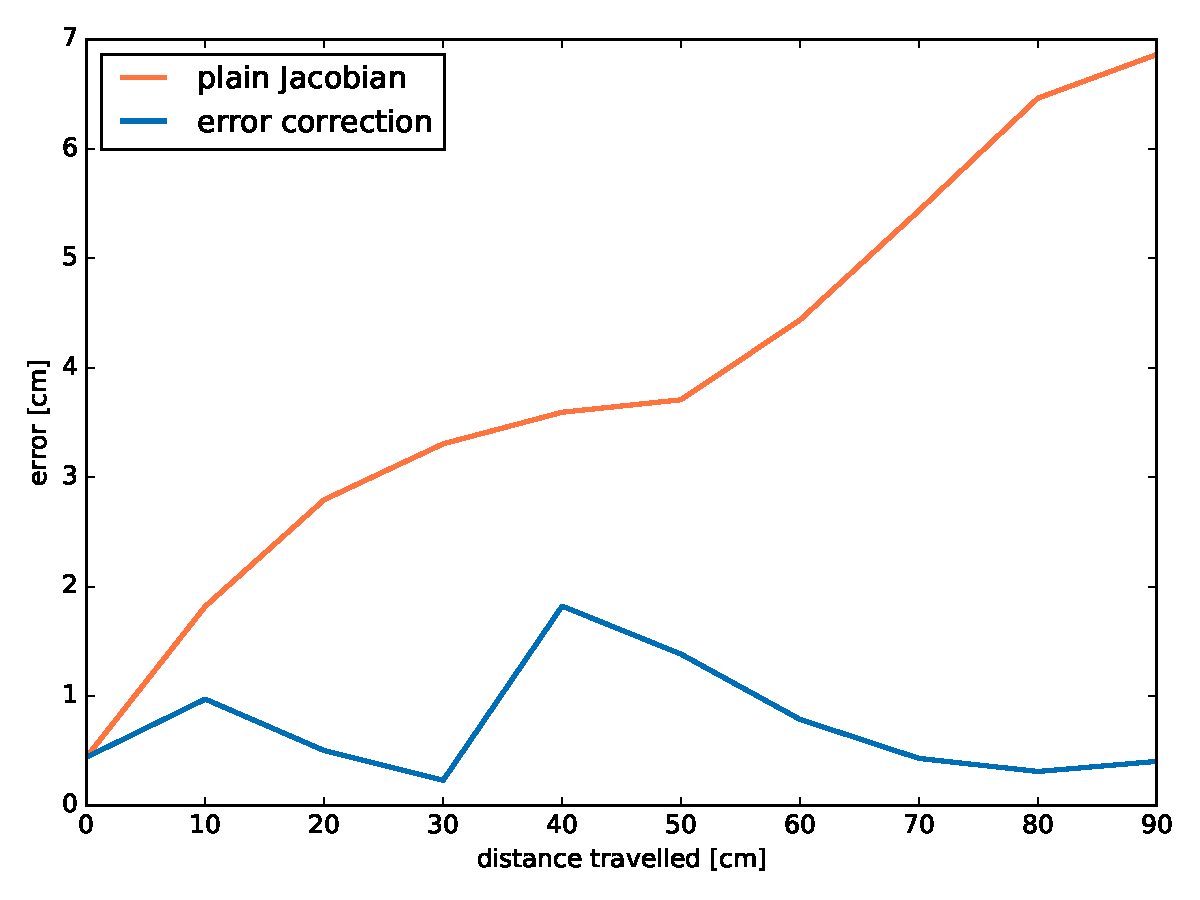
\includegraphics[width=7cm]{jacob_error_real.pdf}
  \caption{Position error during real arm test drive}
  \label{fig:err_jac_real}
\end{figure}

Another issue we noticed was that the movement was in no case as smooth as in the simulator. The arm came to a complete stop every time a decision was made on where to continue. The movement became nearly as jerky as the planned movement. We account this error to the arm dynamics as well, as getting the arm to move seems to take as much time as planning the next step. This could in the future be resolved by splitting the driving and planning into two independent computations, where the next direction would be known even before the arm arrives at the target position. We did not implement the solution due to its implementation complexity.

Overall, we deem the Jacobian control method with error correction fit to be used to drive the robot during exploration, as long as errors caused by singularities are detected and corrected.

With the real arm, we also tested the manufacturer-provided Cartesian speed control. We do not include any quantitative data on the experiment, because the driver failed to fixate the end effector orientation during movement completely, even when zero angular twist was specified. The arm turned in the direction in which it moved. This may be caused by the arm's origin in assistive robotics, where this is the user-expected behavior, similar to the way a human arm moves. It also limits wrist rotation, which seems to be a common source of complications (singularities) when driving the arm, thus making the control less error-prone. Nonetheless, the need to control angular speed such that the orientation does not change renders the feature unusable for our application.

\subsection{Stopping the arm}
\label{subsec:exp_stop}

Another of concerns about whether things will work in the real world was about stopping the arm. Will the arm stop in time? We let the arm touch obstacles that can be moved away if the system failed, and proceeded to tests on real obstacles upon gaining the confidence that the system worked. In Figure~\ref{fig:exp_stop}, the arm can be seen trying to touch a table.

\begin{figure}[ht]
  \centering
  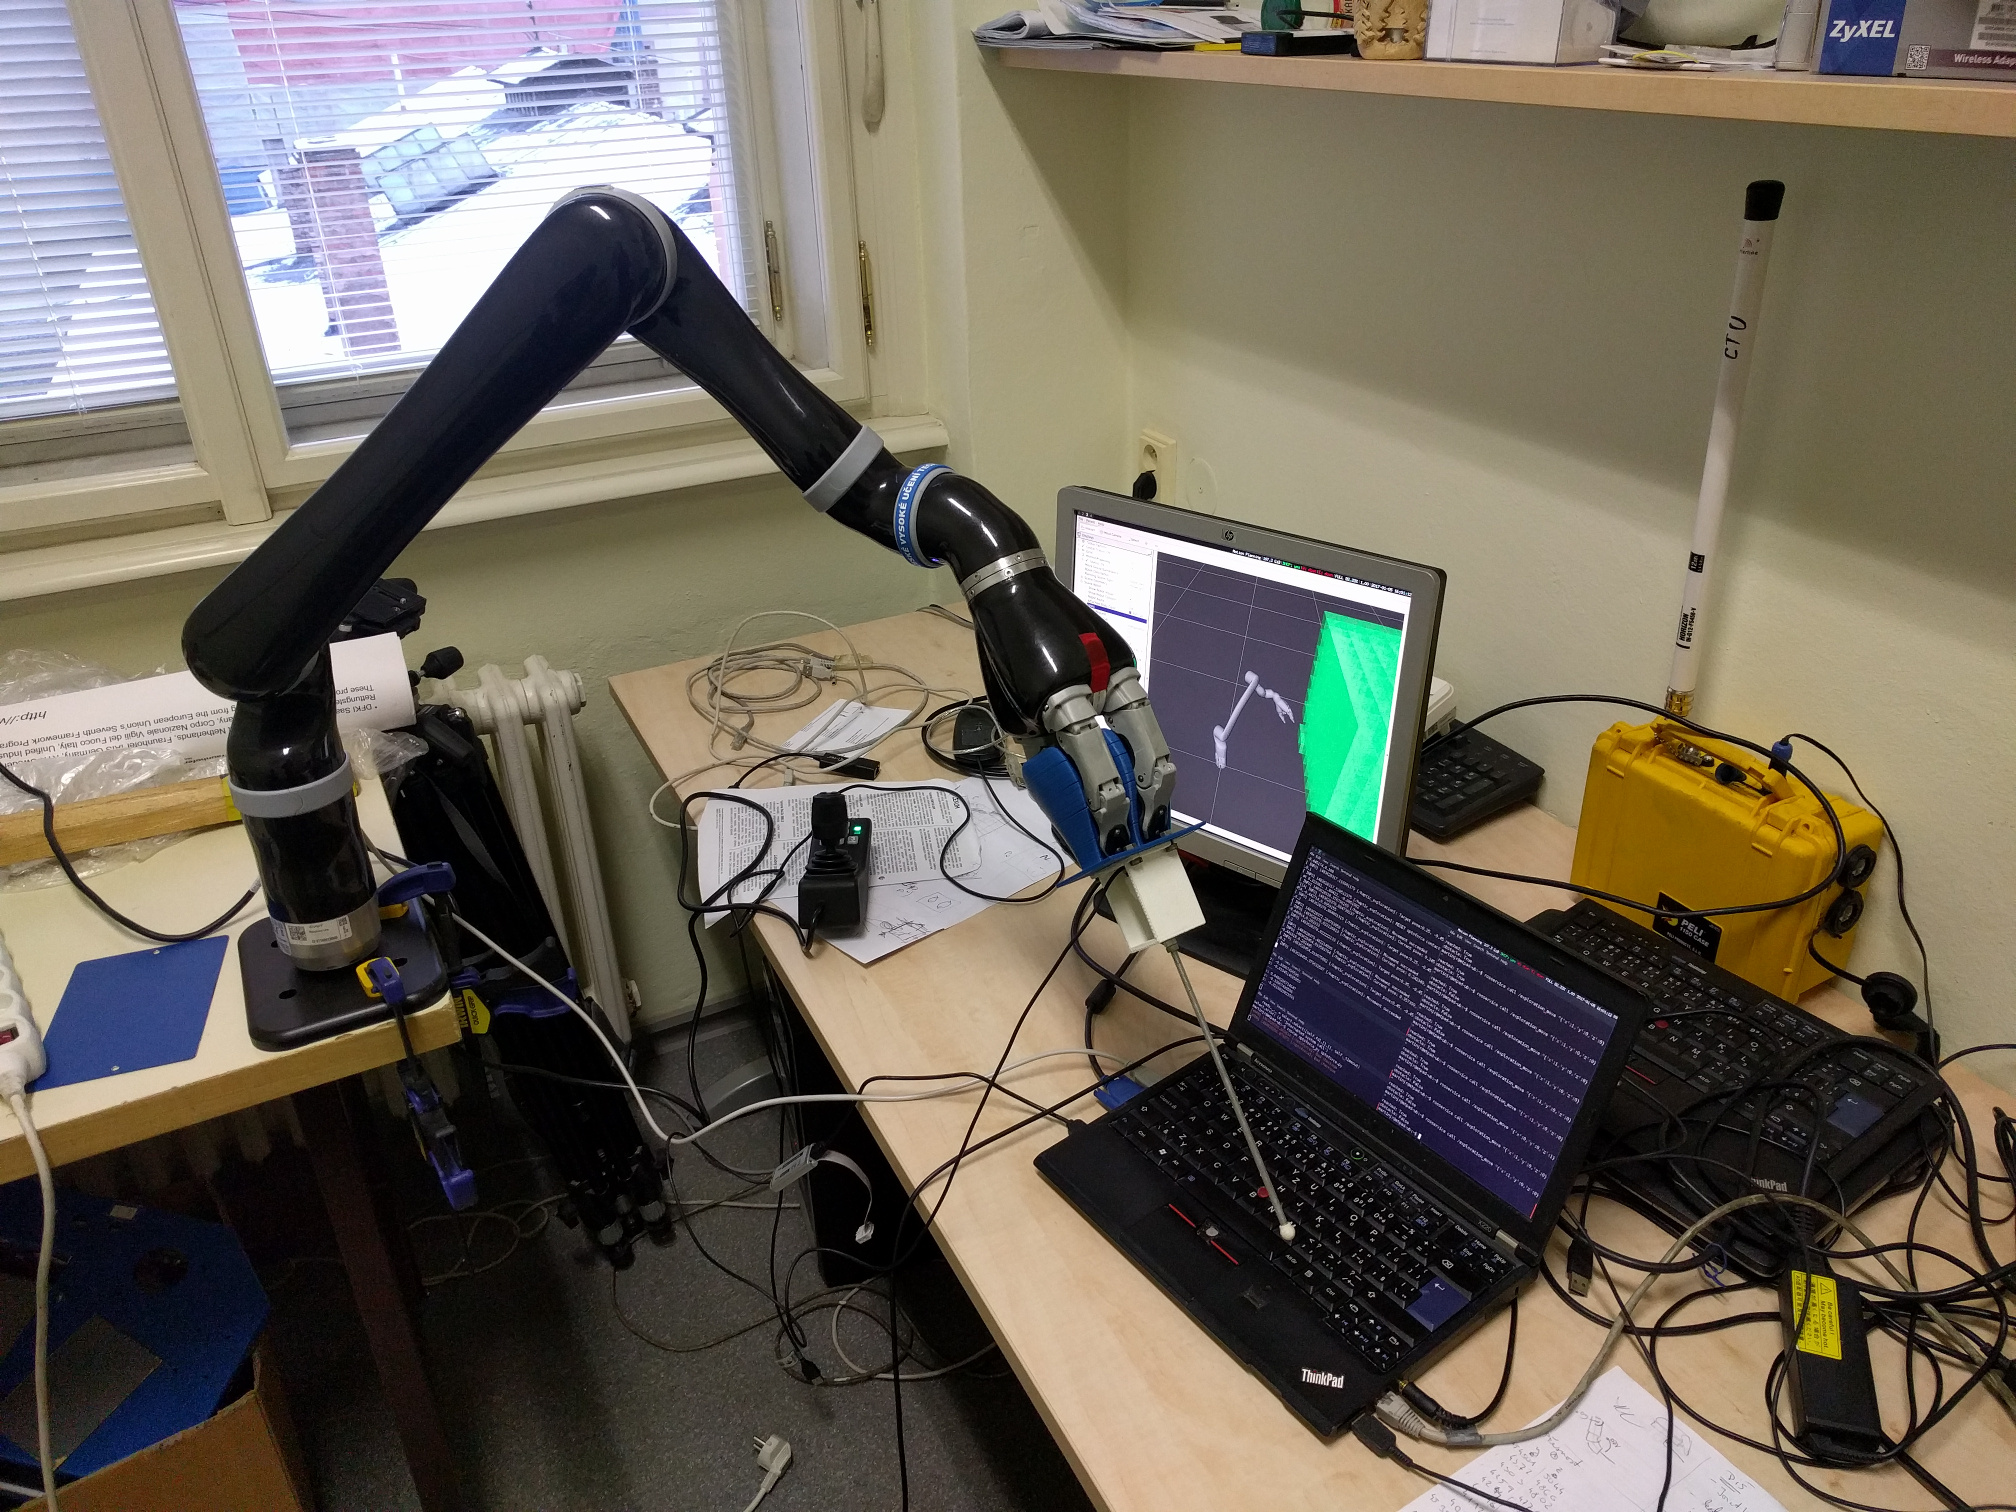
\includegraphics[width=7cm]{photo/exp_real_stopping.jpg}
  \caption{The arm touching a table}
  \label{fig:exp_stop}
\end{figure}

The system latency proved to be low enough to stop the arm in time. After detecting contact (force reading exceeding the threshold), the arm traveled at most another 0.5\,cm with both Jacobian control and planned motion control, corresponding to a delay of 50\,ms with the Jacobian controller. The delay is caused both by latencies in the system and the arm dynamics, where stopping the moving arm takes some time.

The measurement tool has some slack that can absorb the extra movement, and, more importantly, the force sensor is based on deformation, magnified by the stick length, so some extra traveled distance does not pose a problem. The only case in which the extra travel does matter is in case of direct axial contact of the stick with a perpendicular surface. Then, the stick does not have any way to bend and could reach the mechanical hard limit on the tool, perhaps even damage it. When using the tool in this mode, we recommend slowing the arm down so that the latency results in movement of only a few millimeters, tolerable for the tool. Better still, we recommend not to use the tool in this mode, which can be avoided by tilting the tool relative to the direction of motion, thus giving it chance to deform before breaking.



\subsection{Exploring the environment}
\label{subsec:expl_real}

As in the simulated tests, we let the arm explore free space first. Then, we prepared a simple test environment for the arm to explore. Several test runs had to be terminated because of the cable leading to the sensing tool wrapping around the arm links too tightly. This could in the future be resolved by using the data line built into the arm joints, passing all the way through the arm. 

The arm exploring the free space can be seen in Figure~\ref{fig:exp_real_empty}. The exploration showed the same artifacts as in the simulation: when collision checking for the stick was disabled, only five cells in the workspace were misclassified as unreachable (for reasons stated above). The stick would however have traveled through unexplored space many times, leaving room for accidents. 

When the stick was included in the checks, the motion planner failed almost constantly, succeeding only in edge cells of the workspace. This made the algorithm unusable.

\begin{figure}[ht]
  \centering
  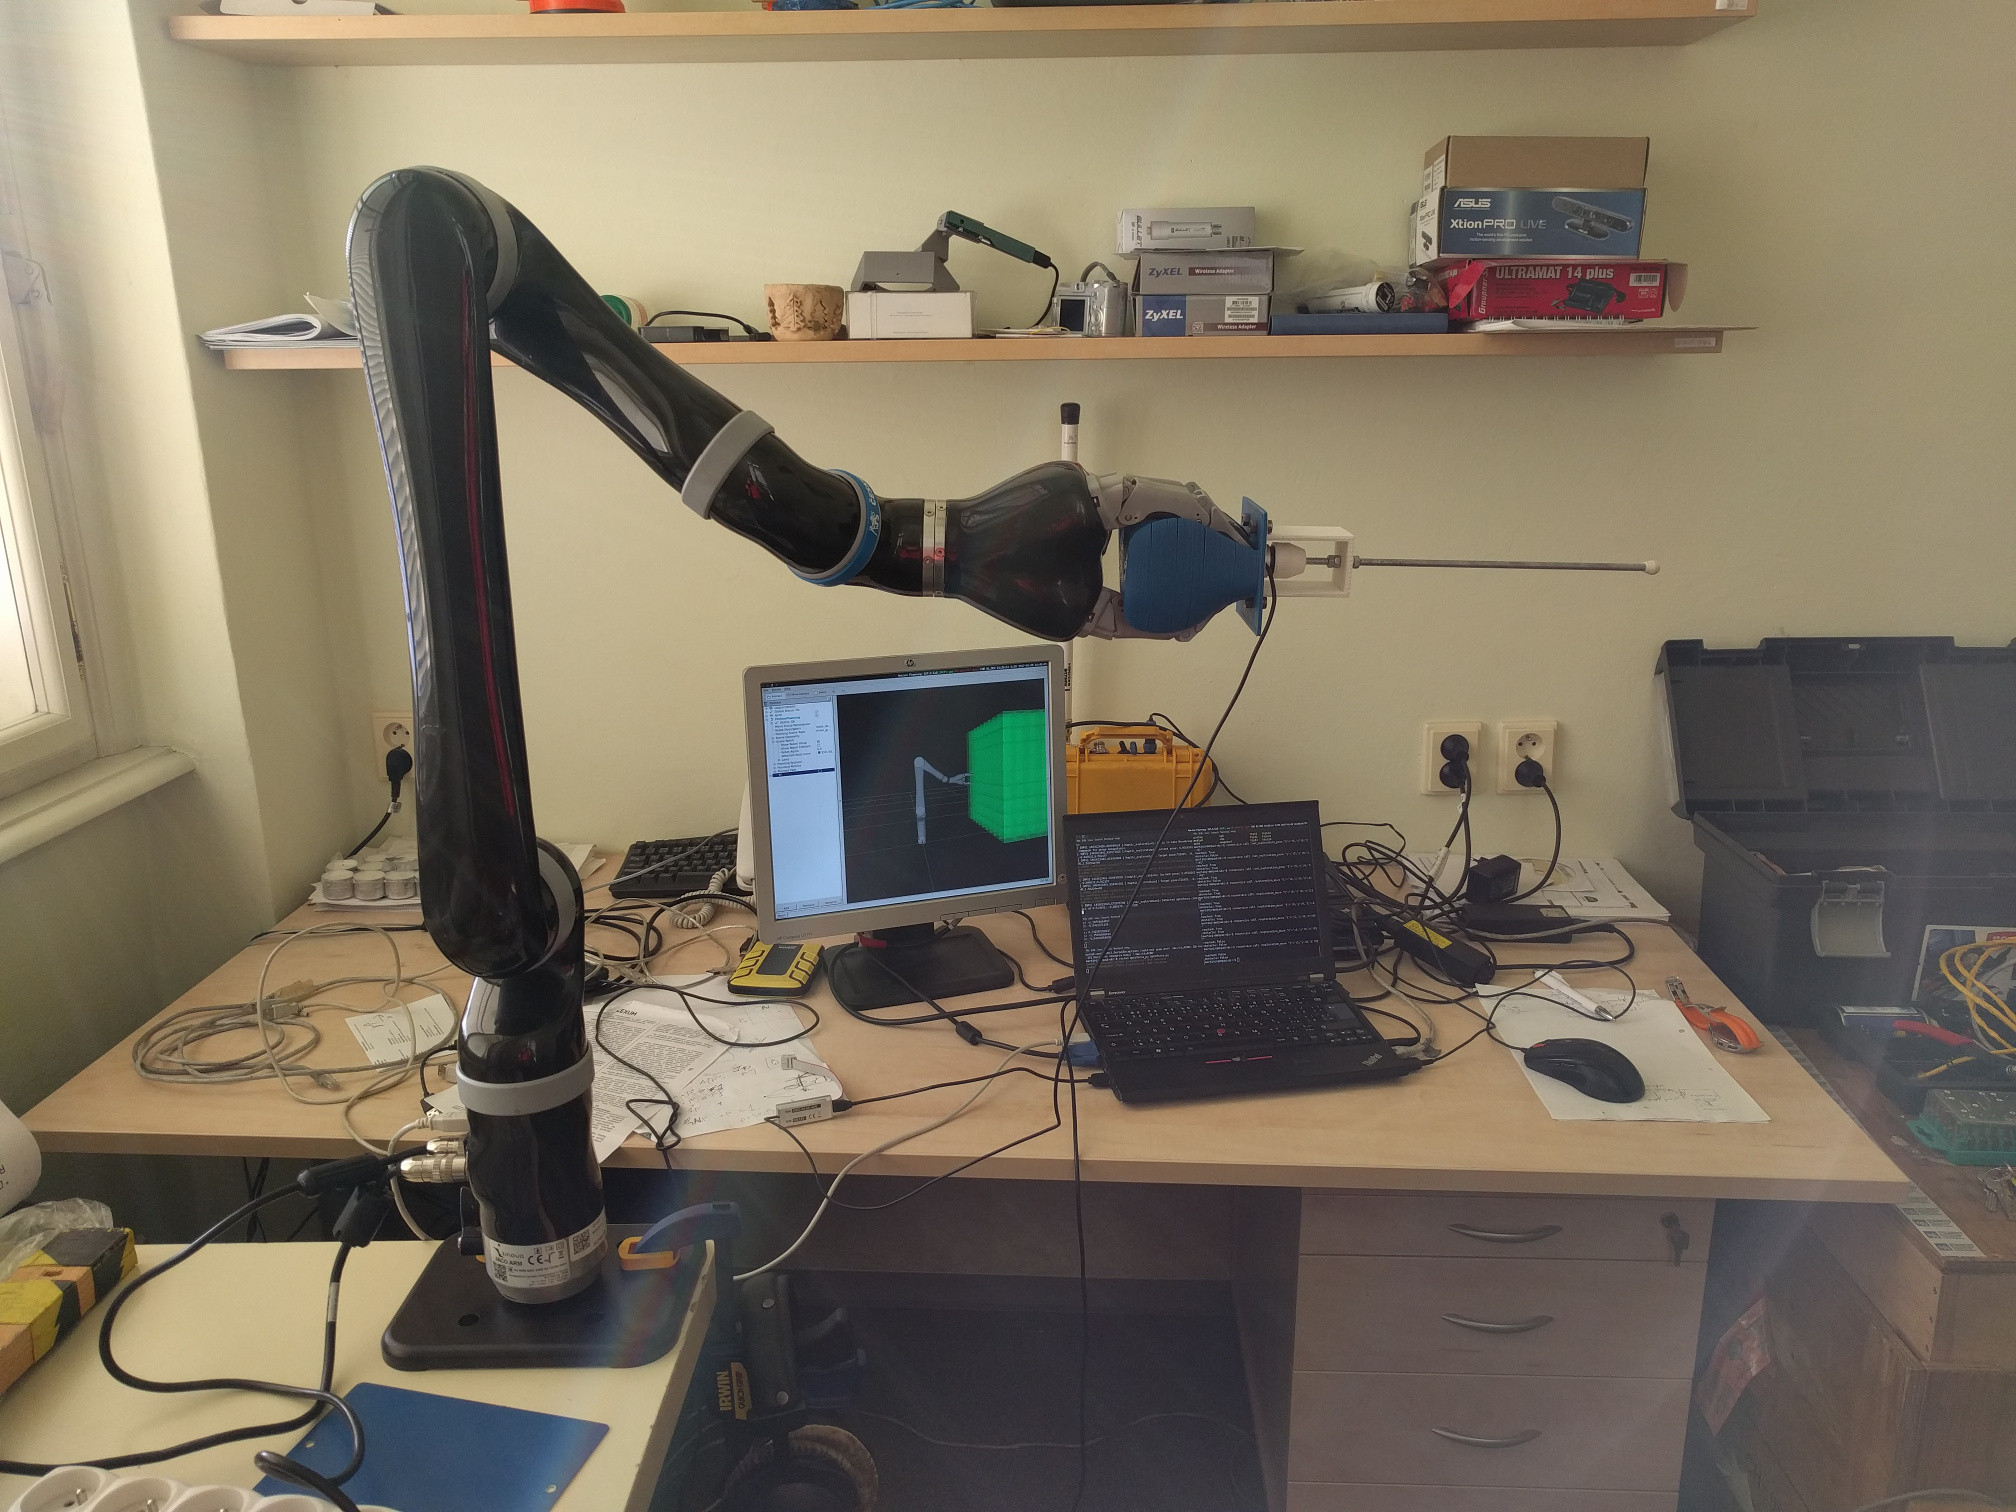
\includegraphics[width=7cm]{photo/exp_real_empty.jpg}
  \caption{The real arm exploring empty environment}
  \label{fig:exp_real_empty} 
\end{figure}

The testing environment for the test run with obstacles is presented in Figure~\ref{fig:exp_real_chair}. It was chosen to be simple, without any tight spaces the arm could get trapped in, and mobile, to allow us to stop the experiment if anything bad happened as we were running the experiment with stick collision checks disabled as well.

\begin{figure}[ht]
  \centering
  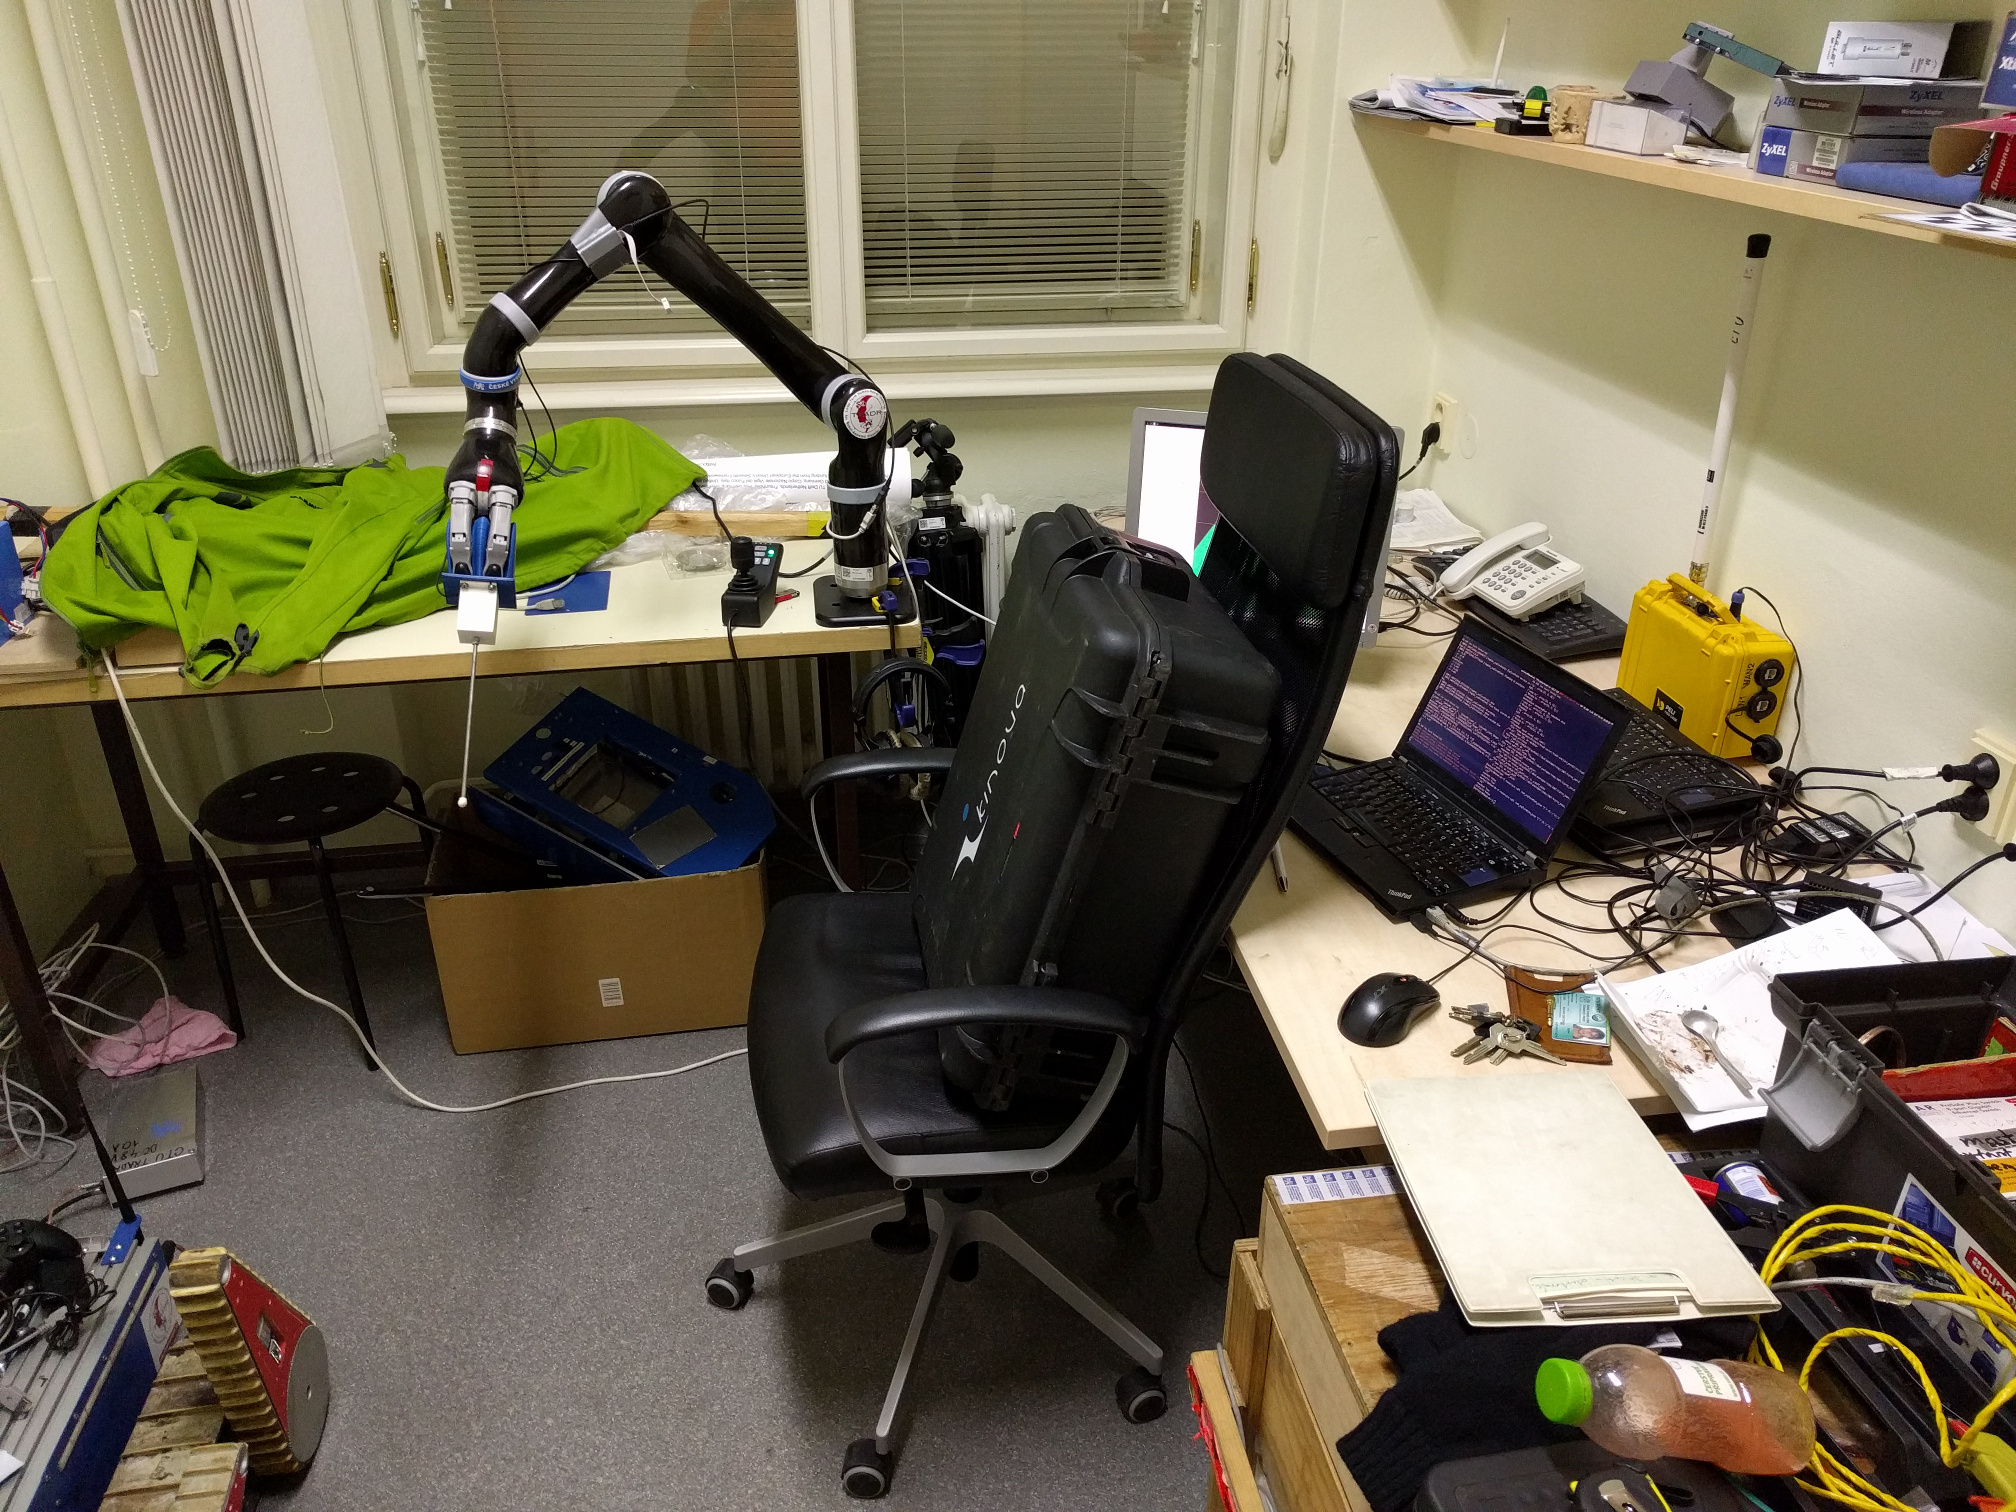
\includegraphics[width=7cm]{photo/exp_real_chair.jpg}
  \caption{The real arm exploring a test environment}
  \label{fig:exp_real_chair}
\end{figure}

During the test run with stick collisions disabled, the exploration went as expected, including the first collisions with the obstacle from the left side as viewed in the picture. Then, after one contact with the obstacle, the arm successfully returned to non-contact position and the exploration algorithm planned a movement to the following cell. A motion plan was successfully found, but it was one of the plans where the arm moves rather wildly before reaching the target. The stick attempted to pass through the obstacle again, stopping the movement and ultimately the whole experiment, as the algorithm detected collision outside the target area.

When we enabled the collision checks for the stick, the arm explored the space safely, never crashing the stick into the obstacle. The same falsely unreachable cells were however reported, and while some space has been successfully marked as empty and some parts of the obstacle were detected, overall, most of the map constituted of unreachable cells.

\subsection{Conclusions}
\label{subsec:label}

The experiments conducted on the real robot verified our ability to steer the arm in empty space. The dynamics the physical arm brings into the equation did not alter the behavior of the algorithm. Around collision objects, the motion planning was not able to compute a collision-free plan, which resulted in reporting unreachable cells just as in the simulated environment. All the suggestions posed in Section~\ref{subsec:exp_sim_concl} apply here: implementing a motion planner more suited for this task would improve the robustness and stability of the whole system.


\end{document}


%%% Local Variables:
%%% mode: latex
%%% TeX-master: "buriama8_dp"
%%% End:
